\begin{figure}[H]
\centering
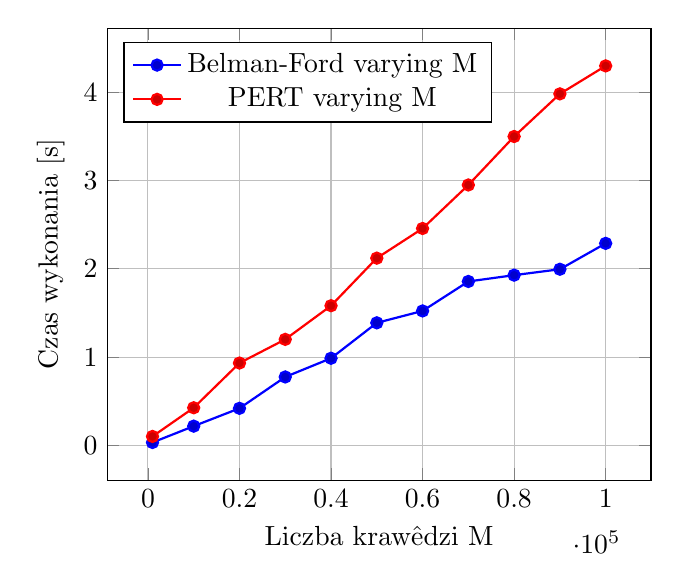
\begin{tikzpicture}
\begin{axis}[
xlabel = {Liczba krawêdzi M},
ylabel = {Czas wykonania [s]},
legend pos = north west,
grid = both,
width = 0.7\linewidth
]
\addplot + [mark = *, thick] coordinates
    {
(1000, 0.03323245048522949)(10000, 0.2181563377380371)(20000, 0.4198935031890869)(30000, 0.7751266956329346)(40000, 0.9867153167724609)(50000, 1.3878788948059082)(60000, 1.5224850177764893)(70000, 1.8562514781951904)(80000, 1.9275805950164795)(90000, 1.9945971965789795)(100000, 2.2875711917877197)};
\addlegendentry
{Belman-Ford varying M}
\addplot + [mark = *, thick] coordinates
    {
(1000, 0.10164165496826172)(10000, 0.4262828826904297)(20000, 0.9326775074005127)(30000, 1.2006115913391113)(40000, 1.5817220211029053)(50000, 2.120281457901001)(60000, 2.456129550933838)(70000, 2.9486136436462402)(80000, 3.497480869293213)(90000, 3.98022198677063)(100000, 4.2970404624938965)};
\addlegendentry
{PERT varying M}
\end{axis}
\end{tikzpicture}
\caption
{Porównanie czasów wykonania algorytmów Belman-Ford i PERT przy stałym N=1000 i różnej liczbie krawędzi M}
\label{fig:time_measurements_m}
\end{figure}
